\documentclass[sigplan,screen,nonacm]{acmart}
\settopmatter{printacmref=false,printccs=false,printfolios=true}
\renewcommand\footnotetextcopyrightpermission[1]{}
\pagestyle{plain}
\emergencystretch=1em

\title{Work Reduction and Memory Optimization for a Finite Abelian Sandpile}
\author{Zicheng Song}
\affiliation{%
  \institution{University of Illinois Urbana-Champaign}
  \department{CS 598 Advanced Performance Engineering}
  \city{Urbana}
  \country{USA}}

\begin{document}
\begin{abstract}
This paper optimizes end-to-end computation of the identity on a
$1001\times1001$ Pacman-shaped Abelian sandpile. Profiling attributes 99.94\%
of sampled baseline time to stabilization. Batch toppling, compact domain
traversal, padded contiguous storage, precomputed geometry, and alternating
sweep direction reduce the three-run median from 611.89~s to 270.22~s, a
2.264$\times$ speedup. The optimized program remains portable and sequential,
and produces output identical to the baseline through the full workload.
\end{abstract}
\maketitle
\hypersetup{pdfauthor={Zicheng Song}}

\section{Introduction and Problem}
An unstable sandpile cell contains at least four grains. A toppling removes
four grains and sends one to each orthogonal neighbor; grains sent outside the
finite domain are lost. Repeated toppling reaches a unique stable state
regardless of toppling order. The assignment computes the group identity on a
finite Pacman-shaped domain by stabilizing an all-six grid, subtracting the
result from six, and stabilizing again. For $N=1001$, this direct computation
is dominated by repeated whole-domain scans. The optimization objective is
therefore to reduce both the number and cost of stabilization visits without
special-casing the requested image.

\section{Baseline and Profiling}
The supplied C baseline stores rows in separate allocations. On every pass it
visits a bounding region, recomputes the circle and mouth predicates, and
performs at most one toppling per unstable visit. It was compiled unchanged
with GCC~15.2.0 and \texttt{-O3 -g -Werror -lm}. On an otherwise-idle Ubuntu
26.04 VM with four Intel Xeon Silver 4216 vCPUs and 15~GiB RAM, three complete
$N=1001$ runs took 609.47, 611.89, and 613.58~s.

Hardware-counter profiling was unavailable: the VM sets
\texttt{perf\_event\_paranoid=4}, so unprivileged \texttt{perf record} and
\texttt{perf stat} fail. I did not alter the system policy. As a fallback, a
\texttt{gprof} run at $N=401$ assigned 99.94\% of sampled time to
\texttt{stabilize} and 0.06\% to PNG compression. Optimization consequently
focused on stabilization rather than rendering or startup.

\section{Optimization Techniques}
\textbf{Batch toppling.} For a cell value $v\ge4$, the optimized code computes
\[
  q=\left\lfloor\frac{v}{4}\right\rfloor,
\]
stores $v-4q$, and adds $q$ to each neighbor. This is algebraically identical
to $q$ consecutive single topplings at the same cell. The Abelian property
permits these operations to be grouped without changing the stable result.

\textbf{Compact domain and precomputed geometry.} The Pacman membership test
depends only on $N$ and the cell coordinates. The final program evaluates it
once, then stores valid cells as row-major linear indices. Stabilization scans
only this list, eliminating repeated circle and mouth tests and avoiding cells
outside the domain.

\textbf{Padded contiguous storage.} One contiguous allocation replaces the
baseline's separately allocated rows. A one-cell zero border surrounds the
grid, so the hot loop can update four fixed offsets without boundary branches.
Updates into the border implement the same sink behavior as grains leaving the
rectangular image. Contiguous storage also improves spatial locality; its cost
is modest extra memory for the border and domain-index list.

\textbf{Alternating sweeps.} Successive passes traverse the compact list in
opposite directions. Toppling order does not affect the final stable state,
but bidirectional propagation reduces the measured $N=401$ sweep count from
22,747 to 21,880.

\section{Experimental Method}
All reported timings are serial, end-to-end \texttt{/usr/bin/time}
measurements, including PNG generation. Each $N=1001$ configuration was run
three times on the same VM; medians are reported. The ablation uses measured
$N=401$ runs to keep comparison practical. Complete outputs are compared by
SHA-256. Smaller tests at $N=1,2,3,4,5,10,31,101,201$ additionally compare
baseline and optimized PNGs and require every domain value to lie in $[0,3]$.

\begin{figure}[t]
  \centering
  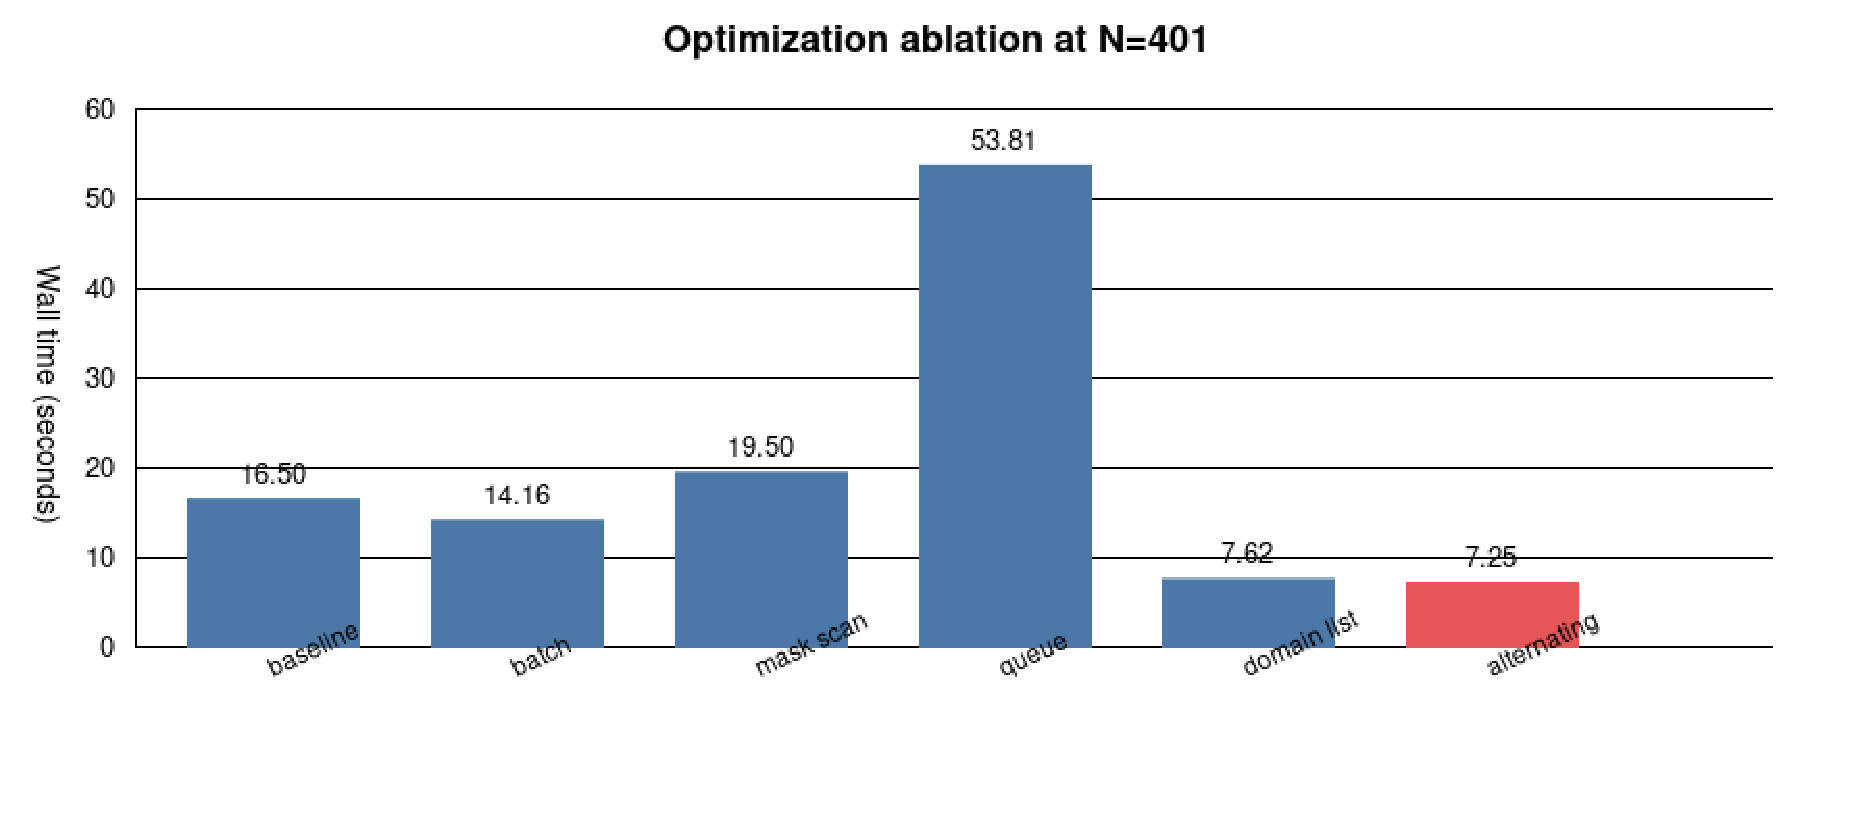
\includegraphics[width=\columnwidth]{../figures/ablation.pdf}
  \caption{Measured end-to-end $N=401$ ablation. Lower is better.}
  \label{fig:ablation}
  \Description{Bar chart of six measured N=401 runtimes: baseline 16.50 seconds,
  batch 14.16, mask scan 19.50, queue 53.81, domain list 7.62, and alternating
  sweep 7.25.}
\end{figure}

\balance
\section{Results and Discussion}
Table~\ref{tab:full} summarizes the full workload. Optimized runs took 270.45,
269.92, and 270.22~s; their median is 270.22~s and range is 0.53~s. Relative to
the 611.89~s baseline median, the speedup is 2.264$\times$. Median peak RSS
increases by 2,308~KiB (18.5\%), from 12,484 to 14,792~KiB.

\begin{table}[t]
  \centering
  \caption{Full $N=1001$ end-to-end comparison.}
  \label{tab:full}
  \begin{tabular}{lrr}
    \toprule
    Metric & Baseline & Optimized \\
    \midrule
    Median time (s) & 611.89 & 270.22 \\
    Time range (s) & 4.11 & 0.53 \\
    Speedup & 1.000$\times$ & 2.264$\times$ \\
    Median peak RSS (KiB) & 12,484 & 14,792 \\
    \bottomrule
  \end{tabular}
\end{table}

Figure~\ref{fig:ablation} separates useful work reduction from plausible but
unhelpful alternatives. At $N=401$, batch toppling improves 16.50 to 14.16~s.
A precomputed full mask regresses to 19.50~s because it still scans all $N^2$
cells. Compact forward traversal reaches 7.62~s, and alternating traversal
reaches 7.25~s. The final $N=1001$ run visits 589,365 domain cells over 132,647
sweeps and performs 37.44 billion unstable-cell visits; stabilization remains
expensive, but each visit is substantially cheaper than in the baseline.

The active-cell queue was also correct but took 53.81~s at $N=401$. It
processed 982,807,074 queue events. Maintaining membership state and enqueuing
neighbors cost more than the stable-cell checks it avoided. This failure shows
that reducing nominal visits does not help when scheduling each visit is too
fine grained; the compact scan instead trades some redundant checks for a
simple, predictable memory-access pattern.

\section{Correctness, Scope, and Introspection}
Every recorded optimized PNG matches its baseline counterpart. Three complete
$N=1001$ baseline and optimized runs share a SHA-256 digest beginning
\texttt{4883dba5}; the artifact retains the full digest.
ASan and UBSan pass at $N=201$. Valgrind at $N=101$ reports zero errors, zero
leaks, and no live allocations at exit.

The transformations assume the assignment's threshold of four, orthogonal
neighbors, finite Pacman geometry, and sink behavior. Batch toppling and
alternating order rely on the Abelian property. Padding is valid because border
values are sinks and are never read back. Geometry construction uses 64-bit
arithmetic, while the hot grid retains the baseline 32-bit representation. The
program accepts arbitrary positive sizes and uses no machine-specific
instructions, but remains sequential and scan based. A future design would
need to reduce propagation iterations without reproducing the queue's
scheduling overhead.

\section{Conclusion}
The dominant cost was not PNG output but repeated stabilization work. Combining
algebraic batching with a compact, contiguous representation and alternating
traversal yields a portable 2.264$\times$ end-to-end speedup while preserving
the exact result. The rejected mask and queue experiments further indicate
that locality and low per-visit overhead matter as much as visit count.

\section*{AI Assistance Disclosure}
An OpenAI coding agent assisted with implementation, remote experiment
automation, testing, data reduction, figure generation, and drafting. All
reported measurements were executed on the stated UIUC VM and are retained in
the artifact.

\end{document}
